\chapter{Hádaj číslo (podmienky)}

Vytvoríme hru, kde bude hráč hádať číslo od 1 do 1000. Opäť si vytvoríme adresáre \code{Assets/Scenes} a \code{Assets/Scripts} a prvú scénu uložíme ako \code{Assets/Scenes/Main.unity}.

Do scény vložíme jeden Text element, jeden InputField a jeden Button. Rozloženie a texty na prvkoch môžu byť napr. ako na obrázku \ref*{fig:plocha_hry_hadaj_cislo}.

\begin{figure}[h]
	\centering
	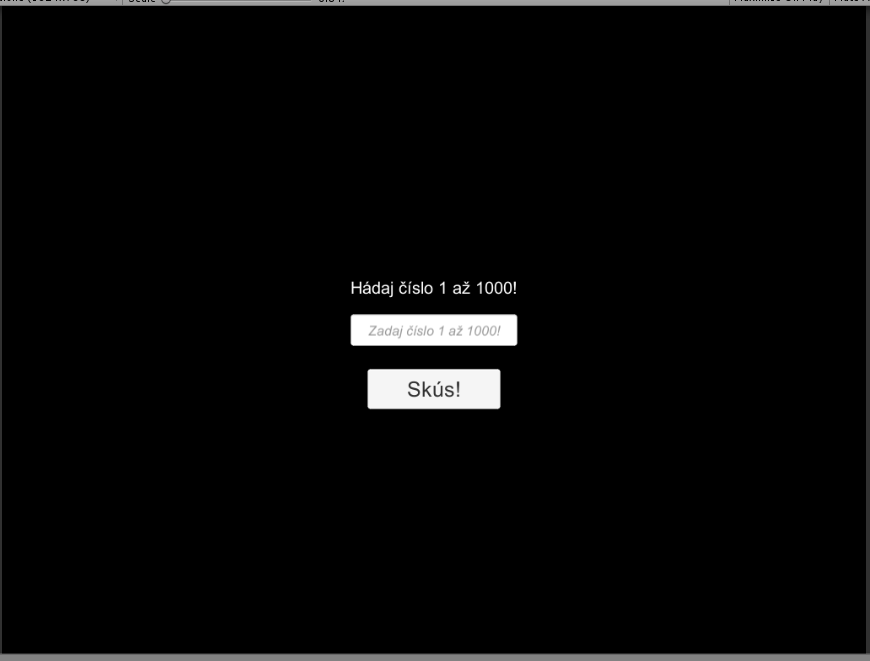
\includegraphics[width=0.98\textwidth]{./graphics/hadaj_cislo/plocha_hry.png}
	\caption{Ukážka rozloženia prvkov.\label{fig:plocha_hry_hadaj_cislo}}
\end{figure}

Vytvoríme skript \code{Assets/Scripts/Hra.cs}. Bude obsahovať odkazy na Text, InputField a Button, z metód bude obsahovať klasický Start, Update môžeme zmazať, NovaHra a jedinu verejnu metodu Testuj. Všetky bez parametrov. NovaHra vygeneruje náhodné číslo medzi 1 a 1000, bude volaná v Start a v Testuj, keď hráč uhádne číslo. Testuj bude kontrolovať vstup z InputField, bude volané z Button-u. Skript môžeme pridať napr. ako komponent pre Canvas (ďalej predpokladám, že je tam). Buttonu pridáme volanie Testuj po kliknutí (ako referenciu zvolíme Canvas). Výsledný kód hry je na \refCode{lst:Hra1}.

\lstinputlisting[language=CSharp,caption=Hotová hra.,label=lst:Hra1]{./codes/hadaj_cislo/Hra_1.cs}